\section{Design}
\begin{figure}
  \centering
  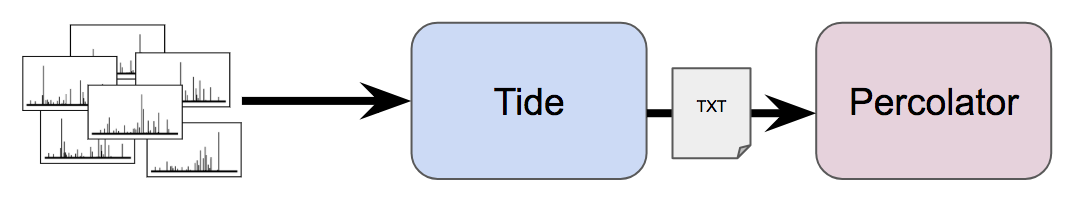
\includegraphics[scale=0.3]{serial_pipeline}
  \caption{Serial Pipeline}
  \label{fig:serial_pipeline}
\end{figure}
\begin{figure}
  \centering
  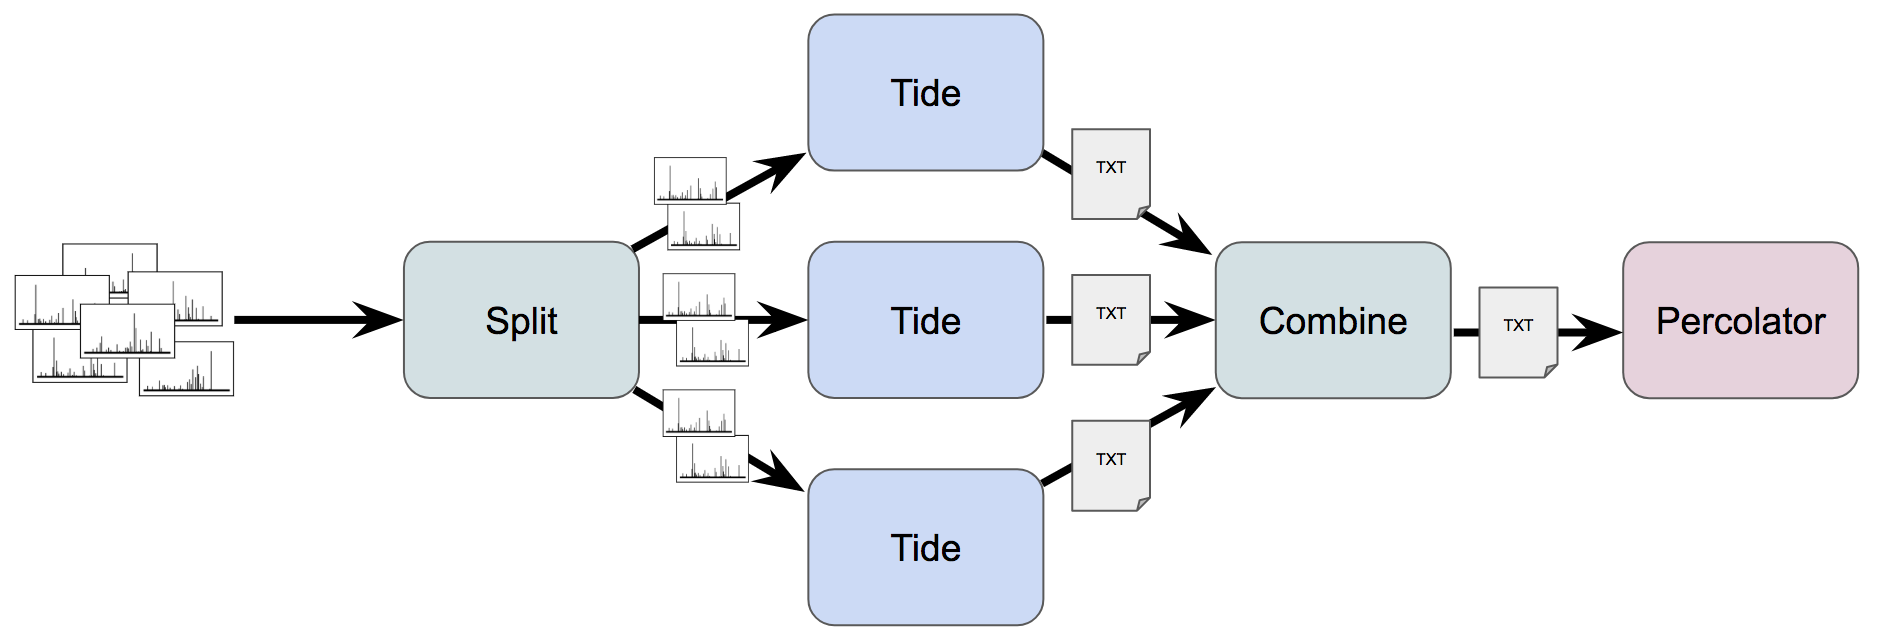
\includegraphics[scale=0.3]{lambda_pipeline}
  \caption{Lambda Pipeline}
  \label{fig:lambda_pipeline}
\end{figure}

The first attempt at designing \name tried to keep the pipeline as serial as possible, like in Figure \ref{fig:serial_pipeline}.
Initially, we used Comet, which is one of the most popular tools to analyze spectra\cite{comet}.
However, Comet was too slow and analyzing just one spectrum took Comet around five minutes in Lambda.
Since Lambda limits task execution time to five minutes, using Comet was not an ideal choice, as analyzing just one spectrum had a high chance of timing out.\\
\newline
Like Comet, Tide analyzes experimental spectra.
Tide creates FASTA database indices which decreases finding potential theoretical spectra matches by 79.5\% to 97.2\%\cite{crux}.
In Lambda, Tide can analyze over 40 thousand spectra in less than 10 seconds.\\
\newline
As shown in Figure \ref{fig:serial_pipeline}, in the serial pipeline, experimental spectra is given to Tide.
Tide processes the spectra and outputs the matches and these matches can be passed to Percolator.

%\\Matching the experimental spectra against theoretical spectra can be extremely slow. To speed up the process, Tide can compute index values for the theoretical spectra and use these indices to speed up the search process.\\

